\documentclass{beamer}
\usepackage{graphicx}
\usepackage{color}

\usetheme{Berlin}
\usecolortheme{beaver}
\title[A constant current applied to the HH model produces a train of action potentials.]{Step current responce of the HH Model}

\author[E.Ioannidis \& J.Hobin] {
   \texorpdfstring{
        \begin{columns}
            \column{.45\linewidth}
            \centering
            Eleftherios Ioannidis\\
            \href{mailto:elefthei@mit.edu}{elefthei@mit.edu}
            \column{.45\linewidth}
            \centering
            James Hobin\\
            \href{mailto:hobinjk@mit.edu}{hobinjk@mit.edu}
        \end{columns}
   }
   {Eleftherios Ioannidis \& James Hobin}
}


\institute{MIT EECS}
\date{\today}

% ============================================
% DOCUMENT BEGINING HERE
% ============================================

\begin{document}

% Title slide (1)
\begin{frame}
  \titlepage
\end{frame}

% slide 2
\begin{frame}
  \begin{figure}
    \centering
    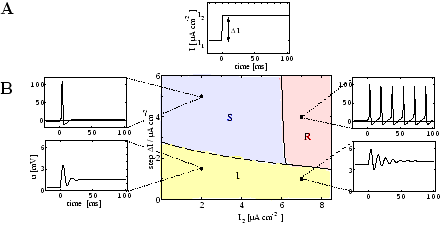
\includegraphics[width = 0.8\textwidth]{./pictures/gerstner.png}
    \caption{Phase diagram for stimulation with a step current.}
  \end{figure}
\end{frame}

% slide 3
\begin{frame}

\end{frame}


\end{document}
